\section{Design(Chris, Sergey)}

CLAS12 Data Aquisition system designed as pipeline-style network-based system. Data taking process starts from front-end components. Those components can have different hardware and software implementation but have to follow certain requirements to be compatible with the rest of the system. Currently front-end components used are commercial VME/VXS crates, commercial Linux servers and JLAB-designed VXS Trigger processor boards. VTPs installed in VXS crates but read out by DAQ as independent components. All components are running on 250MHz clock discributed over optic fibers. The same fiber system is used to disctibute syncreset and trigger signals and to collect busy signals from all front-end electronics.

All front-end components are connected to Event Builder (EB) which is multi-threaded program running on multi-core Linux server. Most connections are 1Gbit ethernet links. For several components generating significant data rate 10Gbit ethernet connection is used.

Complete events are sent to Event Transfer (ET) System. ET is multi-threaded program providing data ring where various data processing programs can be attached to monitor data quality online. It can be run on the same server as EB, or can be used to create sequensial chain of servers to increase data processing power.

Last component in data chain is Event Recorder (ER). It is multi-threaded program receiving data from ET system and recording it to the disk. Multi-stream mode is available, allowing to write several files in parallel to the same or different disk partitions to burst writing performance. Event order in multi-stream mode is preserved.

CLAS12 DAQ System diagram is shown on Fig.~\ref{fig:DAQdiagram}.

\begin{figure}[hbt]
	\centering
	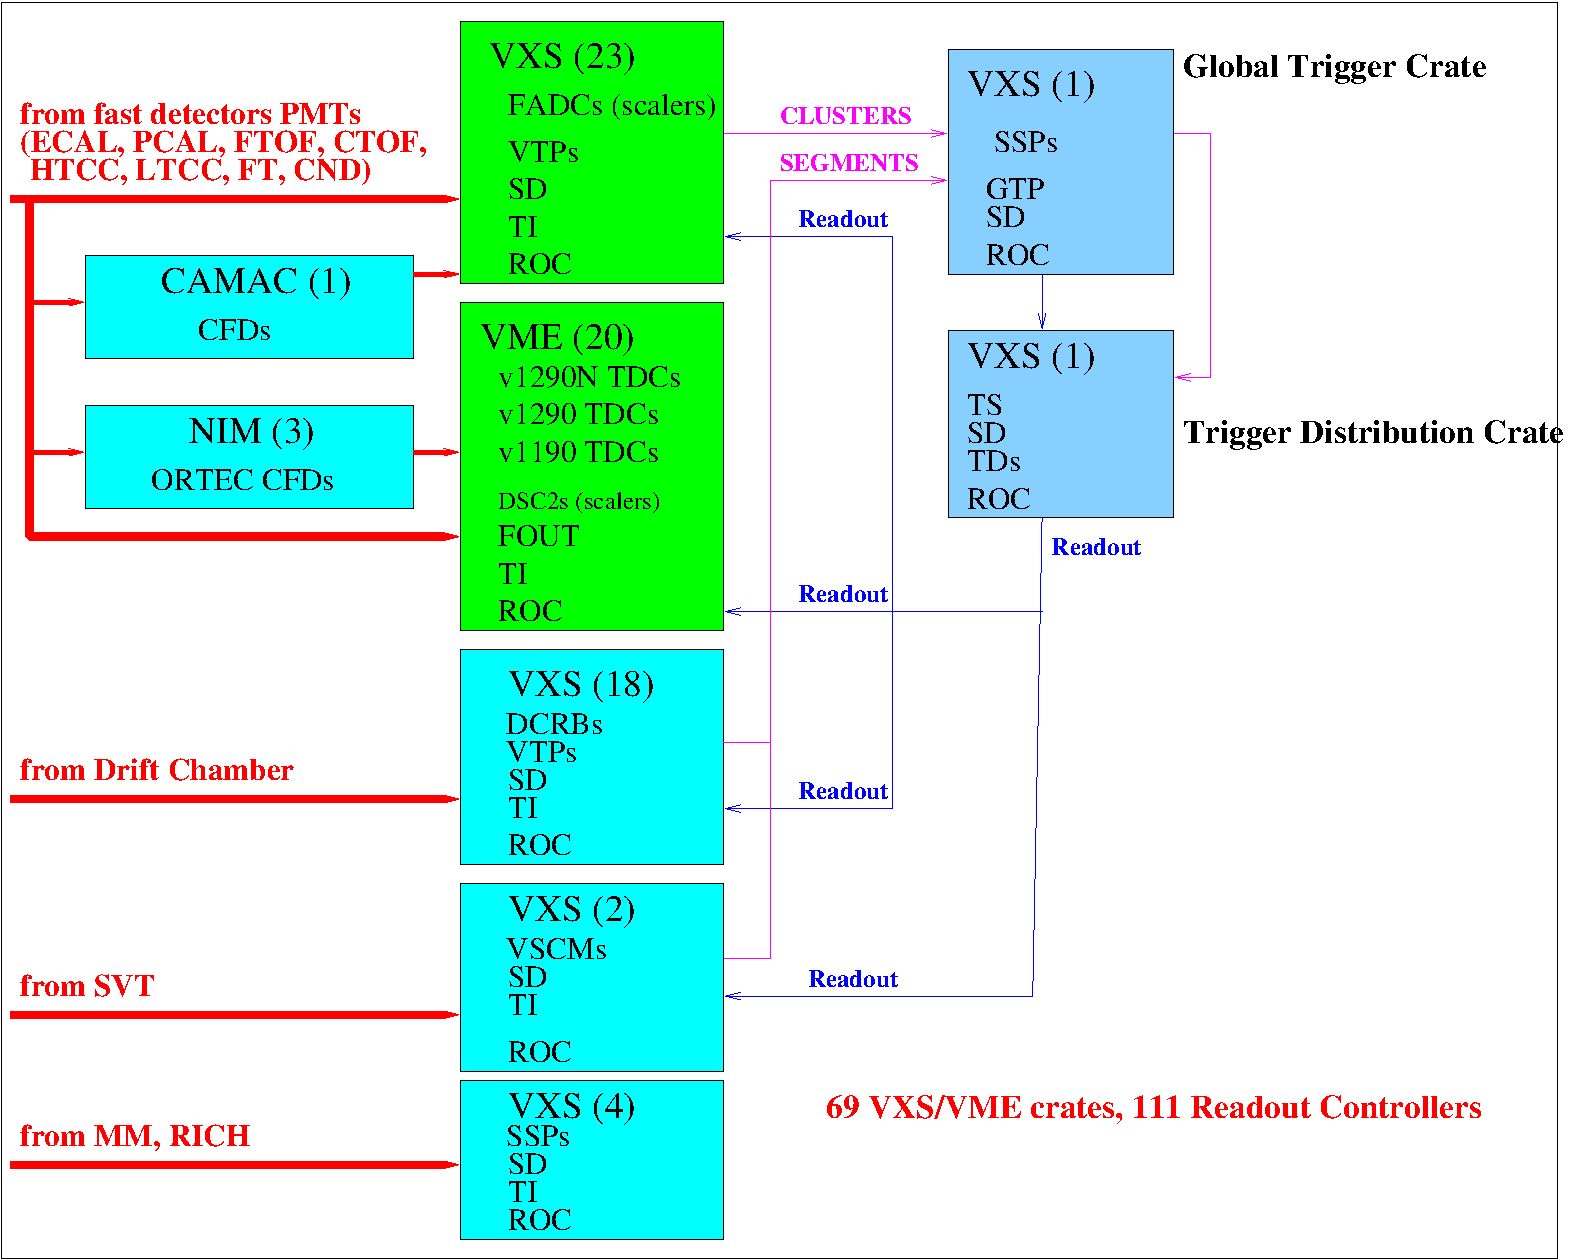
\includegraphics[width=1.0\columnwidth,keepaspectratio]{img/CLAS12_HARDWARE_2.pdf}
	\caption{CLAS12 Data Aquisition System Diagram}
	\label{fig:DAQdiagram}
\end{figure}

